%!TEX root = thesis.tex"`

\chapter{\Gls{pipeline} обучения}
\begin{figure}[h]
    \centering
    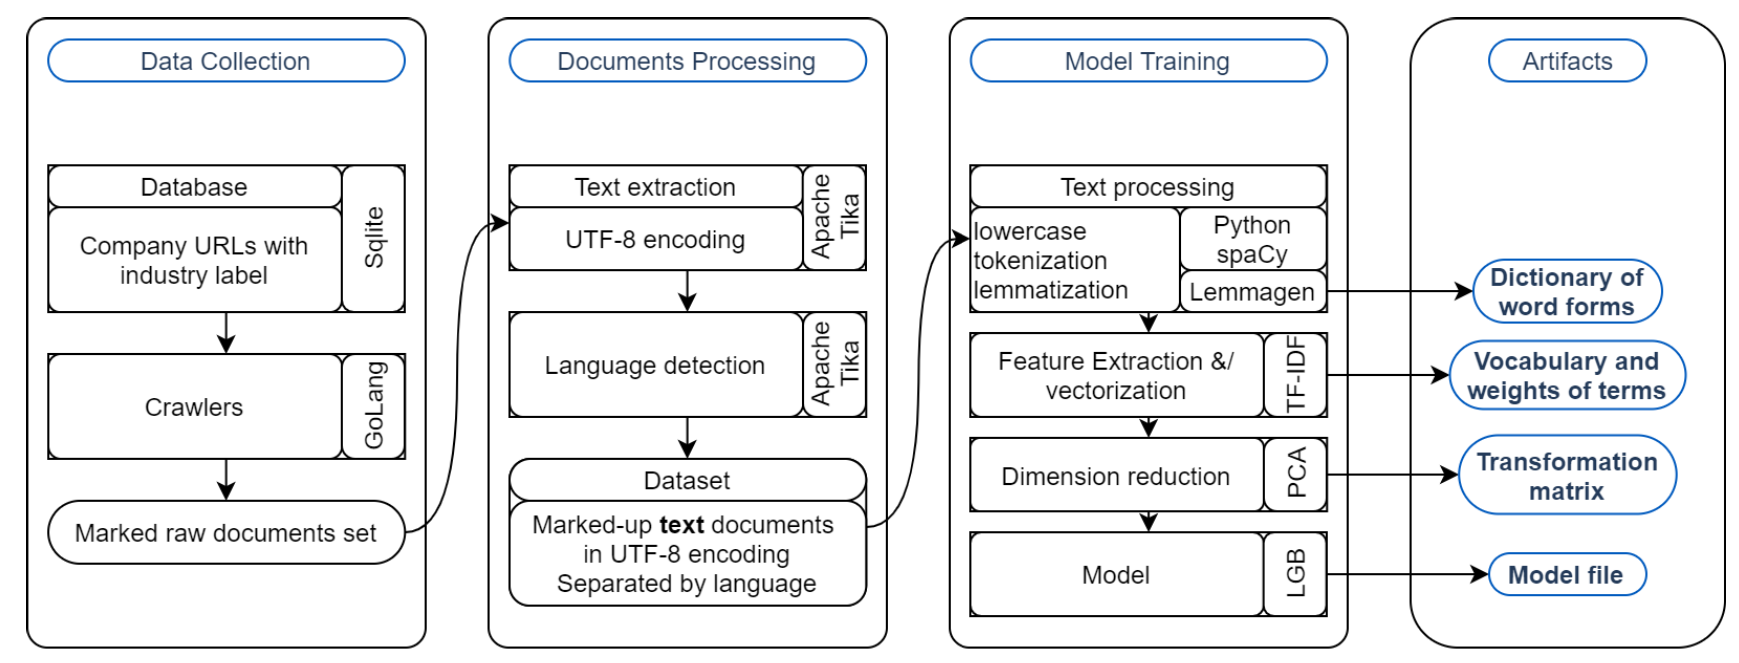
\includegraphics[width=\linewidth]{pipeline}
    \caption{Схематичное изображение процесса обучения}
    \label{fig:pipeline}
\end{figure}

Процесс обучения состоит из трех стадий:
\begin{enumerate}
    \item Сбор данных (data collection), см. \ref{sec:data-mining}.
    \item Обработка (processing) собранных документов, см. \ref{sec:preprocessing}.
    \item Обучение модели и сохранение артефактов, см. \ref{sec:training}.
\end{enumerate}
Каждая из этих стадий будет раскрыта подробнее в дальнейших секциях.

\section{Структура данных}
\subsection{Сырые данных}
В настоящей работе в качестве входных данных выступают документы, выгруженные из открытых источников в сети Интернет.
Данные представляют из себя веб-страницы, сохраненные локально в разнообразных форматах (HTML, PDF, .doc и другие).
Сопутствующий мультимедийный контент (видеозаписи, аудизаписи, картинки и т.п.) не сохраняется и не учитвается в модели.
Любой язык разметки, метаинформация, скрипты и таблицы стилей (в случае HTML) сохраняются в сырых документах <<как есть>>.

Все документы, участвующие в процессе, делятся на категории.
Категории заранее фиксированы и размечаются вручную.
Ниже приведен их список:
\label{categories}
\begin{itemize}
    \item Sales, Marketing and PR
    \item HR
    \item Finance and Banking
    \item IT, IT research and Development
    \item Manufacturing
    \item Medical and Paramedical
    \item Business and Corporate
    \item Legal
    \item Others
\end{itemize}

Разметка сырых данных фиксируется на уровне веб-сайта, т.е. \textbf{все} документы одного веб-сайта относятся к одинаковой категории.
Такой способ разметки является приближенным, поскольку один и тот же веб-сайт может содержать документы, относящиеся к различным тематикам (к примеру, медицинский сайт может содержать помимо мед.документов образцы договоров об оказании платных услуг).
\subsection{Данные для обучения}
Модель классификатора реализована на очищенных и нормализованных документах.
Данные для обучения представляют из себя набор файлов (по одному на каждую категорию из \ref{categories}), каждый из которых содержит множество документов.

Каждый документ в таком файле представляет из себя одну строку, которая заполнена словами в свой начальной форме, разделенными пробелом.
В таком формате данные предстают в человекочитаемом виде и то же время могут быть легко обрабтаны компьютером.

\section{Получение сырых данных}
\label{sec:data-mining}
\subsection{Общее описание \gls{crawler}}
\begin{wrapfigure}{r}{7cm}
    \centering
    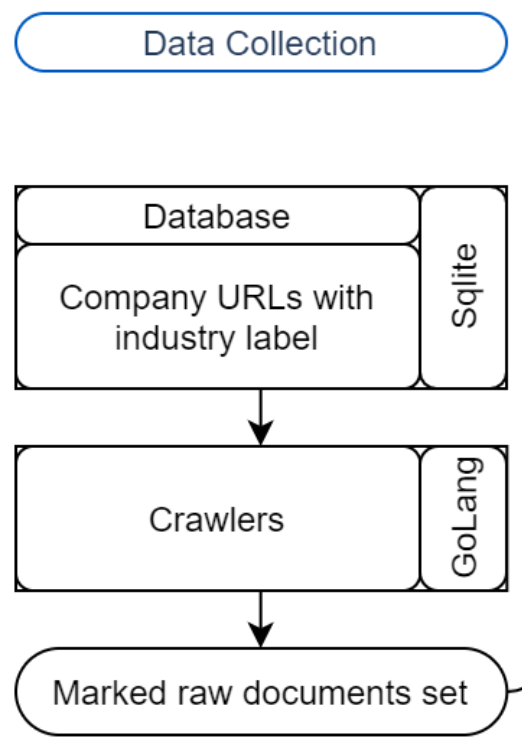
\includegraphics[width=\linewidth]{crawlers-pipeline}
    \caption{Архитектура \gls{crawler}}
    \label{fig:crawler-pipeline}
\end{wrapfigure}
Для получения документов была разработана программа для выгрузки веб-страниц (\gls{crawler}).
Для достижения большей производительности \gls{crawler} был написан на языке \gls{golang}, сочетающим высокую скорость работы и относительную простоту написания кода.

Схематично архитектура краулера показана на рис. \ref{fig:crawler-pipeline}.
На каждую поддерживаемую локализацию заводится своя база данных, содержащая ссылки сайтов, сгруппированные по категории.
Категории сайта записываются в базу данных вместе с множеством URL-адресов - пример этого изображен на рис. \ref{fig:crawler-db-head}.
Такая БД содержит немного данных, поэтому для простоты интеграции с \gls{golang} в качестве \acrshort{dbms} используется \gls{sqlite}.

\begin{figure}[h]
    \centering
    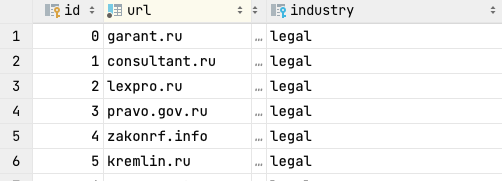
\includegraphics[width=0.8\linewidth]{crawler-db-head}
    \caption{Пример данных из БД краулера}
    \label{fig:crawler-db-head}
\end{figure}
Файл с заполненной базой данных поступает на вход программе \gls{crawler} (второй большой прямоугольник на \ref{fig:crawler-pipeline}), который запускет обход в глубину каждого URL-адреса.
В каждом выгруженном веб-сайте ищутся все возможные гиперссылки на другие страницы, и эти гиперссылки добавляются в очередь выгрузки.
Процесс продоложается до тех пор, пока вся очередь выгрузки для данного сайта не будет исчерпана, либо не будет достигнут лимит на количество загружаемых документов с одной страницы (\crawlerPageLimit).
\subsection{Типы используемых \gls{crawler}}
Существует несколько типов краулеров и подходов к их реализации \cite{cite:crawler-review}.
Помимо этого на стороне сайта возможно применение методов защиты от автоматической выгрузки \cite{cite:crawler-protection}.
Это, с одной стороны, создает некоторую вариативность, а с другой стороны -- обязывает иметь запасные варианты реализации сбора данных с веб-страниц.
С учетом данных факторов в настоящей работе используется три типа \gls{crawler}: \textit{google crawler}, \textit{colly crawler} \cite{cite:colly} и \textit{common index crawler} \cite{cite:common-crawl}.

Google \gls{crawler} напрямую запрашивает все документы с сайта через веб-поисковик \url{https://google.com}.
Этот метод весьма эффективен, т.к. полагается на собираемый Google индекс сайтов, но в то же время очень ограничен, т.к. \url{google.com} достаточно быстро начинает запрашивать CAPTCHA при запросе.
Обойти проверку CAPTCHA возможно несколькими способами, описанными, к примеру, в \cite{cite:captcha-bypass-1} и \cite{cite:captcha-bypass-2}.
Однако все эти способы требуют большие вычислительные мощности, что не удовлетворяло требованию о быстрой работе краулера.
Поэтому были разработы другие краулеры.

Common Index \gls{crawler} запрашивает копию страницы из интернет-архива \href{https://commoncrawl.org/}{Common Crawl}.
Это -- самый безотказный способ, т.к. веб-архив не требует ввода CAPTCHA и имеет нестрогие ограничения на количество запросов.
Тем не менее, архив может содержать не все страницы и скорость загрузки может быть ограничена из-за технических особенностей платформы.

Colly \gls{crawler} \cite{cite:colly} является самым продвинутым из описанных краулеров.
В то время как остальные \gls{crawler} полагаются на сторонние ресурсы, colly самостоятельно проходит по всем сайтам, выискивая все возможные гиперссылки на другие документы и проходя по ним в следующей итерации.
Такой алгоритм приводит к тому, что выгружаются практически все документы с сайта (кроме тех, что защищены авторизацией или проверками на ботов).
К сожалению, на больших сайтах алгоритм может достаточно долго блуждать по гиперссылкам.
Более того, нет никакой гарантии, что полученный граф обхода не содержит циклов, поэтому colly crawler может потенциально уйти в вечный цикл.
Для защиты от указанных проблем в данном \gls{crawler} выставлен лимит на время выполнения (\collyTimeLimit) и суммарный размер выгружаемых документов (\collySizeLimit).

Использование всех трех краулеров показало хорошие результаты -- по каждому языку было выгружено около 30 Gb сырых документов, что составило порядка 200 тысяч документов.

\section{Преобразование сырых данных в данные для модели}
\label{sec:preprocessing}
% TODO: (ruapyyj) рассказ про тику и tokenizer <- Fri Apr 15 01:22:24 2022
% TODO: (ruapyyj) сравнение spacy и расскажи, как перевел все на nltk ради скорости <- Fri Apr 15 01:22:24 2022

\section{Модель \acrshort{ml} и ее обучение}
\label{sec:training}
% TODO: (ruapyyj) просто обзор, т.к. в модель ты почти не лез <- Fri Apr 15 01:22:51 2022
